% Build with: xelatex definition-of-ox.tex; makeindex definition-of-ox; xelatex definition-of-ox.tex (twice)
\documentclass[11pt,oneside,openany]{book}
\usepackage[letterpaper,margin=1.08in,headheight=14pt]{geometry}
\usepackage{fontspec}
\IfFileExists{/usr/share/fonts/truetype/ebgaramond/EBGaramond12-Regular.ttf}{%
  \setmainfont[Path=/usr/share/fonts/truetype/ebgaramond/,UprightFont=EBGaramond12-Regular.ttf,BoldFont=EBGaramond12-Bold.ttf,ItalicFont=EBGaramond12-Italic.ttf,BoldItalicFont=EBGaramond12-Italic.ttf]{EBGaramond12-Regular.ttf}%
}{\setmainfont{TeX Gyre Pagella}}
\setsansfont{DejaVu Sans}
\setmonofont[Scale=0.83]{DejaVu Sans Mono}
\usepackage{microtype}
\usepackage{amsmath,amssymb,mathtools,mathpartir}
\usepackage{booktabs,longtable,array,tabularx,multicol}
\usepackage{enumitem}
\usepackage{listings}
\usepackage{xcolor}
\usepackage{fancyhdr}
\usepackage{titlesec}
\usepackage{hyperref}
\usepackage{bookmark}
\usepackage{imakeidx}
\usepackage{needspace}
\usepackage{tikz}
\usepackage{float}
\makeindex[title=Index,columns=2]
\definecolor{ink}{HTML}{202326}
\definecolor{subtle}{HTML}{5D666B}
\definecolor{rulec}{HTML}{9A9FA2}
\definecolor{shade}{HTML}{F4F5F4}
\definecolor{codec}{HTML}{124F51}
\hypersetup{colorlinks=true,linkcolor=ink,urlcolor=codec,pdfauthor={E. Alvarez and GPT-6},pdftitle={The Definition of ox},pdfsubject={Working formal specification of the ox data-oriented scripting language}}
\lstdefinelanguage{oxlang}{
  morekeywords={val,rec,datatype,of,case,if,then,else,do,end,true,false,andalso,orelse,div,mod,o},
  sensitive=true,
  morecomment=[l]{\#},
  morecomment=[s]{(*}{*)},
  morestring=[b]",
}
\lstset{language=oxlang,basicstyle=\ttfamily\footnotesize,keywordstyle=\bfseries\color{codec},commentstyle=\itshape\color{subtle},stringstyle=\color{codec},backgroundcolor=\color{shade},frame=single,framerule=.24pt,rulecolor=\color{rulec},columns=fullflexible,keepspaces=true,showstringspaces=false,breaklines=true,breakatwhitespace=true,xleftmargin=5pt,xrightmargin=5pt,aboveskip=9pt,belowskip=9pt,tabsize=2}
% Alias with no space in identifier; revised below to keep LaTeX package input forgiving.
\colorlet{codec}{teal!65!black}
\titleformat{\chapter}[display]{\normalfont\bfseries\huge}{\filleft\color{subtle}\Large\thechapter}{9pt}{\huge}
\titlespacing*{\chapter}{0pt}{-10pt}{27pt}
\titleformat{\section}{\normalfont\bfseries\Large}{\thesection}{.7em}{}
\titleformat{\subsection}{\normalfont\bfseries\large}{\thesubsection}{.7em}{}
\pagestyle{fancy}
\fancyhf{}
\fancyhead[L]{\footnotesize\sffamily THE DEFINITION OF ox}
\fancyhead[R]{\footnotesize\sffamily WORKING DRAFT 0.1.2}
\fancyfoot[C]{\thepage}
\renewcommand{\headrulewidth}{.35pt}
\renewcommand{\chaptermark}[1]{}
\newcommand{\ox}{\textit{ox}}
\newcommand{\kw}[1]{\texttt{#1}}
\newcommand{\nt}[1]{\mathit{#1}}
\newcommand{\meta}[1]{\textsf{#1}}
\newcommand{\state}{\sigma}
\newcommand{\env}{\rho}
\newcommand{\judge}[3]{\langle #1,#2\rangle\Downarrow #3}
\newcommand{\pending}{\textbf{Design obligation.}\ }
\newcommand{\impl}{\textbf{Implementation status.}\ }
\newcommand{\ruleline}{\vspace{4pt}\noindent\rule{\linewidth}{.35pt}\vspace{5pt}}
\setcounter{tocdepth}{2}
\setlist[itemize]{topsep=3pt,itemsep=2pt}
\setlist[enumerate]{topsep=3pt,itemsep=2pt}
\begin{document}
\emergencystretch=2em
\frontmatter
\thispagestyle{empty}
\begin{center}
\vspace*{1.3in}
{\Large\sffamily\MakeUppercase{A language definition}}\\[.6in]
{\fontsize{43}{49}\selectfont\bfseries The Definition of \ox}\\[.18in]
{\Large An ML-derived, data-oriented scripting language}\\[.7in]
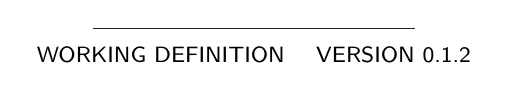
\begin{tikzpicture}
\draw[ink,line width=0.6pt] (-2.05,0)--(2.05,0);
\node[font=\footnotesize\sffamily] at (0,-.33) {WORKING DEFINITION \quad VERSION 0.1.2};
\end{tikzpicture}\\[.9in]
{\Large E. Alvarez \quad and \quad GPT-6}\\[.2in]
{\normalsize Joint language design and formal specification}\\
\vfill
{\large 23 November 2026}\\[7pt]
{\small A specification for the Advent of Code development edition}\\[.22in]
{\small Status: \textbf{proposed}; not a claim of complete implementation}
\end{center}
\clearpage
\chapter*{Preface}
\addcontentsline{toc}{chapter}{Preface}
A precise definition is useful not because a small language must be complicated, but because a small language should have few surprises. \ox{} is intended for scripts which read data, construct explicit domain values, transform those values through ordinary functions, and carry out operating-system effects deliberately. Its surface notation draws from Standard ML; its implementation is being developed in OxCaml.

This book follows the \emph{organization}, not the prose, of Milner, Tofte, and Harper's \emph{The Definition of Standard ML} (1989). The original separates the syntax, static semantics, and dynamic semantics of a Core language, treats modules independently, defines programs, and provides derived forms, a full grammar, and initial bases in appendices. We adopt that architecture on a smaller scale. The supplied Standard ML Definition is our principal reference for the methodological choice. \cite{milner1989}

\paragraph{Status and authority.} This is a \emph{working definition}, not a report that every rule is already implemented. Sections explicitly distinguish \textbf{normative proposals} from \textbf{implementation status} and \textbf{open design obligations}. A rule in this document states intended \ox{} behavior; it does not silently certify the current interpreter. When the proposed definition differs from the current seven-file interpreter (through Patch 010), the difference is noted in Appendix E.

\paragraph{A compact thesis.} Data is represented before it is manipulated. Functions are values which transform data. Imperative effects---file reads, process execution, mutable arrays, and tables---remain available and explicit. Object-oriented method dispatch, classes, and inheritance are absent. The ability to execute a script with \texttt{\#!/usr/bin/env ox} is a language-level requirement.

\paragraph{Authorship.} This is a collaborative design by E. Alvarez and GPT-6. The human collaborator may revise the displayed author name in the LaTeX source before formal publication. No claim is made that GPT-6 is a legal person or a copyright owner.

\tableofcontents
\clearpage
\mainmatter

\chapter{Introduction}
\section{Purpose}
The purpose of \ox{} is to provide a small, data-oriented scripting language suitable for operating-system automation and short computational exercises such as Advent of Code. It is not a POSIX shell, not a Standard ML implementation, and not a general-purpose optimizing compiler.

An \ox{} program is a sequence of declarations. Those declarations introduce values, recursive functions, and algebraic datatype constructors. Effects are invoked through built-in functions such as \kw{U.read}, \kw{U.write}, \kw{Process.run}, and \kw{P.printf}; arbitrary external commands are not implicitly interpreted as syntax.

\section{The three phases}
As in the Standard ML Definition, a program is understood through three phases:
\begin{enumerate}
\item \emph{Parsing} establishes the program's syntax and source locations.
\item \emph{Elaboration} resolves names and checks those static requirements which \ox{} supports.
\item \emph{Evaluation} computes values and performs explicit effects.
\end{enumerate}
These are logically distinct even when a first implementation combines the second and third phases. The initial \kw{ox check} command currently guarantees parsing only; it does \emph{not} establish type safety, termination, absence of effects, or exhaustiveness.

\section{The three levels}
The definition is divided into Core, Modules, and Programs. \emph{Core} contains values, functions, patterns, datatypes, and expressions. \emph{Modules} is a deliberately restricted namespace facility used first for a fixed prelude. \emph{Programs} concerns scripts, process arguments, command-line entry points, and generated context. Unlike full Standard ML, \ox{} 0.1 defines neither user-authored structures nor functors.

\section{A representative program}
\begin{lstlisting}
#!/usr/bin/env ox

datatype turn = Left of int | Right of int

val movement = (turn) =>
  case turn of
      Left clicks => -clicks
    | Right clicks => clicks

val advance = (state, turn) =>
  do
    val moved = state.position + movement turn;
    val position = (moved mod 100 + 100) mod 100;
    val stops = state.stops + (if position == 0 then 1 else 0);

    { position
    , stops
    }
  end
\end{lstlisting}
The record is the result of the computation, not a container of procedures. \kw{movement} and \kw{advance} are ordinary values whose values are functions. A separate script section may read input and print results.

\section{Normative notation}
We use $e$ for expressions, $p$ for patterns, $d$ for declarations, $v$ for values, $\env$ for lexical environments, and $\state$ for externally visible mutable state. An evaluation judgment
\[
\langle \env,\state,e\rangle\Downarrow\langle \state',v\rangle
\]
means that evaluating $e$ in environment $\env$ and state $\state$ terminates with value $v$ and state $\state'$. These judgments describe successful terminating computations; runtime errors are discussed separately.

\chapter{Syntax of the Core}
\section{Reserved words}
The following words are reserved in the proposed Core:
\begin{center}
\begin{tabular}{lllllll}
\kw{val}&\kw{rec}&\kw{datatype}&\kw{of}&\kw{case}&\kw{if}&\kw{then}\\
\kw{else}&\kw{do}&\kw{end}&\kw{true}&\kw{false}&\kw{andalso}&\kw{orelse}\\
\kw{div}&\kw{mod}&\kw{o}&&&&
\end{tabular}
\end{center}
The tokens \kw{fun}, \kw{fn}, \kw{let}, \kw{in}, \kw{switch}, and \kw{breaksw} have no grammatical function. In Patch 010, recursion moved from the former \kw{val rec} declaration syntax to an optional \kw{rec} modifier placed at the function site: \kw{val f = rec (x) => e}.

\section{Special constants}
The initial constants are decimal integers, decimal floating-point literals, double-quoted strings, booleans, and the unit expression \kw{()}. The range of an integer is the host runtime's native tagged integer range unless a future specification defines arbitrary precision. A floating literal has the implementation's supported binary floating representation. Strings are byte sequences; their encoding is not inferred from syntax.

The language recognizes the escapes \verb|\n|, \verb|\t|, \verb|\r|, \verb|\"|, and \verb|\\|. No implicit interpolation takes place within a string. \kw{"a b"} is always one string value, not two process arguments.

\section{Comments}
A leading \kw{\#!} line is treated as a script interpreter directive and ignored by the parser. \kw{\#} introduces a comment to the end of a line. Parenthesized comments \kw{(* ... *)} may nest. Lexical comments do not alter the scope of identifiers.

\section{Identifiers}
Ordinary value identifiers begin with a lowercase letter or underscore. Constructor and module identifiers begin with an uppercase letter. Subsequent characters may be letters, digits, or underscores. \kw{L.map} is a qualified prelude lookup; \kw{state.position} is a record-field projection. Neither denotes an object-method call.

\section{Lexical analysis}
Whitespace separates tokens except within strings. Comments are discarded while source positions are retained. Multi-character operators (including \kw{|>}, \kw{==}, \kw{/=}, \kw{::}, \kw{->}, \kw{=>}, \kw{<=}, and \kw{>=}) take precedence over their constituent characters. A newline is not a statement terminator. Consecutive declarations in \kw{do} blocks are separated by semicolons. A single \kw{=} is reserved for bindings, declarations, and labeled record fields, never comparisons.

\section{Infix operators}
\begin{center}
\small
\begin{tabularx}{\linewidth}{@{}l l X@{}}
\toprule
From looser to tighter & Associativity & Meaning \\
\midrule
\kw{|>} & left & forward application \\
\kw{orelse}, \kw{andalso} & left & short-circuit Boolean operations \\
\kw{o} & right & function composition \\
\kw{==}, \kw{/=}, comparisons & non-associative & equality, inequality, ordering \\
\kw{@} & right & list concatenation \\
\kw{::} & right & list construction \\
\kw{+}, \kw{-}, \kw{\^} & left & arithmetic and string concatenation \\
\kw{*}, \kw{/}, \kw{div}, \kw{mod} & left & multiplication, division, remainder \\
\emph{unary} \kw{-} & prefix & numerical negation \\
function application, projection & left & application and field selection \\
\bottomrule
\end{tabularx}
\end{center}
The proposed grammar will prohibit chained comparisons without parentheses. The Patch 008 grammar handles comparisons as single non-recursive productions; the interpreter still requires OxCaml build validation. Decimal integer \kw{div} and \kw{mod} are specified by truncating quotient and corresponding remainder, not by an implicit Euclidean normalization; an algorithm needing a nonnegative remainder must normalize explicitly.

The operator \kw{|>} is left associative and evaluates its left operand before its right operand. Composition \kw{o} constructs a function and does not execute either component until the composition is applied.

\section{Function parameters and local transformations}
Every function receives one value. Parameter patterns are parenthesized in the
surface language: \kw{(x) => e} denotes a unary function and
\kw{(x, y) => e} takes one tuple value. The form
\kw{(x) -> (y) => e} is \emph{curried}: its first application yields a second
function. Its meaning is two nested unary functions, not one function with
multiple positional arguments. Longer chains associate to the right.

\paragraph{Two distinct arrows.} The token \kw{->} separates parameter levels
in a function expression; the final token \kw{=>} introduces the function body.
The same \kw{=>} still separates a \kw{case} branch pattern from its expression.
In future type annotations \kw{->} may also denote the function-type
constructor; expression and type grammar contexts distinguish these uses.
The absence of \kw{fn} removes no expressive power, but parentheses on
individual parameter levels are mandatory.

\paragraph{Recursive function expressions.} The syntax
\kw{val name = rec (p) => e} assigns a recursive function to \kw{name}.
Curried recursion may use \kw{val name = rec (p) -> (q) => e}. The \kw{rec}
modifier is permitted only immediately after \kw{=} in a \emph{named} value
declaration. It is not a freely usable anonymous recursive expression.

\paragraph{Programming convention.} Prefer one tuple argument for a domain
transformation whose inputs form one conceptual product; prefer currying when
partial application is intended. Compute named intermediate values in a
\kw{do ... end} block before constructing the result or advancing recursion.
\begin{lstlisting}
val count_invalid = rec (rule, current, upper, total) =>
  if current > upper then total
  else
    do
      val is_invalid = invalid (rule, current);
      val contribution = if is_invalid then current else 0;
      val next_total = total + contribution;

      count_invalid (rule, current + 1, upper, next_total)
    end
\end{lstlisting}
The final expression is the block result; semicolons terminate local
declarations rather than recursive calls.

\section{Derived forms}
We distinguish the surface language from a smaller kernel. Record punning, forward application, composition, list displays, and \kw{if} are derived forms. \kw{val f = rec (p) => e} is a special initializer form, not an ordinary lambda value, because the declaration requires recursive lexical scope. Precise translations appear in Appendix A.

\section{Grammar}
Core declarations are value and datatype bindings; a named value declaration may have a recursive function initializer. The core expressions are constants, variables, applications, records, collections, functions, cases, conditionals, and local \kw{do} blocks. Appendix B gives the full proposed surface grammar in EBNF-like notation. The grammar is normative at the level of accepted phrases, not at the level of a particular Menhir conflict-resolution strategy.

\section{Syntactic restrictions}
\begin{enumerate}
\item The same record label may not occur twice in a record expression or record pattern.
\item A pattern may not bind the same variable twice.
\item A \kw{rec} initializer is only permitted directly after the equals sign in a named \kw{val} binding and must be an arrow function; it cannot initialize an arbitrary pattern binding. This prevents arbitrary recursive cyclic data.
\item A \kw{case} expression must contain at least one branch; patterns are tested in source order.
\item Every declaration in a \kw{do} block ends in \kw{;} and the block ends in one result expression followed by \kw{end}.
\item User code does not redefine reserved words. Duplicate constructor names in the same datatype declaration are rejected.
\end{enumerate}
An unreachable or incomplete match should be a static diagnostic where provable. A runtime match failure remains defined for unchecked code.

\chapter{Syntax of Modules}
\section{Scope}
Unlike full Standard ML, \ox{} 0.1 exposes a \emph{closed prelude namespace}. The initial namespace contains long names such as \kw{List.filter}, together with short aliases such as \kw{L.filter}. These are references to the same builtin functions, not copies or methods.

\section{Module identifiers}
A module identifier is a capitalized name. A qualified selection has the form \kw{Module.name}. The parser may represent it using the same projection syntax as \kw{record.field}; resolution distinguishes namespace values from user records through the lexical environment.

\section{Initial namespaces}
\begin{center}
\begin{tabular}{lll}
\toprule
Long name & Short name & Domain \\
\midrule
\kw{List} & \kw{L} & immutable lists \\
\kw{Array} & \kw{A} & mutable arrays \\
\kw{String} & \kw{S} & string transformations \\
\kw{Printf} & \kw{P} & formatted output \\
\kw{Unix} & \kw{U} & filesystem and environment \\
\kw{Int} & \kw{I} & integer utilities \\
\kw{Table} & \kw{T} & mutable keyed storage \\
\kw{Process} & --- & external processes \\
\kw{Path} & --- & paths and globbing \\
\bottomrule
\end{tabular}
\end{center}
\section{Excluded module syntax}
The tokens \kw{signature}, \kw{structure}, \kw{struct}, \kw{sig}, and \kw{functor} are not in the 0.1 surface grammar. Their implementation would enlarge the type and module systems without advancing the immediate scripting goal. Named prelude namespaces remain extensible in a future edition; this definition neither promises functor application nor silently incorporates OxCaml's module syntax.

\section{Namespace restrictions}
A module lookup fails if the module or selected member is absent. \kw{L.map} denotes an ordinary function value. Expressions of the form \kw{x:method(...)} are not admitted. Record projection and module selection are syntactically similar but semantically never imply implicit receiver arguments.

\chapter{Static Semantics for the Core}
\section{Simple objects}
Let $\mathsf{Var}$ be ordinary identifiers, $\mathsf{Con}$ constructor names, and $\mathsf{Lab}$ record labels. We use a constructor stamp $\kappa$ to distinguish constructors created by different datatype declarations, even if their textual names coincide. These are semantic objects, not syntax available to scripts.

\section{Compound objects}
Proposed types $\tau$ are generated by
\[
\tau ::= \mathtt{unit}\mid\mathtt{bool}\mid\mathtt{int}\mid\mathtt{float}\mid\mathtt{string}
\mid \tau\;\mathtt{list}\mid\tau\;\mathtt{array}\mid\tau_1\times\tau_2
\mid \{\ell_i:\tau_i\}_{i=1}^n\mid\tau_1\to\tau_2\mid t.
\]
Here $t$ is a user-defined datatype. A dynamic runtime may carry values of all these types without checking every judgment statically.

\section{Projection, injection, and modification}
A record type is a finite mapping from labels to types. Projection $\{\ldots,\ell:\tau,\ldots\}.\ell$ has type $\tau$. Constructor injection maps a payload to a member of a declared sum type. Mutable array/table modification changes the store, not a lexical \kw{val} binding.

\section{Types and type functions}
The proposed type notation for lists, products, and datatype payloads follows ML practice. The surface grammar permits declarations such as \kw{datatype turn = Left of int | Right of int}. It does not yet expose arbitrary user type aliases or polymorphic type parameters as a release requirement.

\section{Type schemes}
\pending Full Hindley--Milner generalization, principal types, and the Standard ML value restriction are not requirements of \ox{} 0.1. We reserve the notation $\forall\alpha.\tau$ for a possible later static checker but make no principal-typing claim in this edition.

\section{Scope of identifiers}
A declaration extends only the subsequent lexical environment in its containing scope. In \kw{do val x = e; body end}, the new $x$ is visible in $body$ but not outside the block. Ordinary \kw{val x = e} evaluates $e$ in the old environment. In \kw{val f = rec (p) => e}, $f$ is in scope while its closure is formed.

\section{Non-expansive expressions}
A literal, lambda, or data constructor may be side-effect-free in isolation. By contrast, \kw{U.read}, \kw{Process.run}, and mutable table operations are effects. This classification informs future effect diagnostics but is not a purity type system: \kw{val} does not promise that its initializer is pure.

\section{Closure and binding}
Let $\Gamma$ map variables to types or to the untyped marker $\mathsf{dynamic}$. Bindings are lexically scoped. A closure carries its defining environment. Captured state may include references to mutable arrays and tables, so closure creation does not imply deep immutability.

\section{Type environments}
A datatype declaration introduces a type name and constructors. A constructor \kw{Left of int} has the logical signature $\mathtt{int}\to\mathtt{turn}$, while a nullary constructor \kw{Done} is a value of its datatype. Prelude namespaces contribute predefined symbols to the initial environment.

\section{Inference and checking rules}
For a future sound static subset, we use $\Gamma\vdash e:\tau$ as a typing judgment. Representative rules are:
\begin{mathpar}
\inferrule*[right=Variable]{\Gamma(x)=\tau}{\Gamma\vdash x:\tau}
\and
\inferrule*[right=Function]{\Gamma,x:\tau_1\vdash e:\tau_2}{\Gamma\vdash ((x)\Rightarrow e):\tau_1\to\tau_2}
\and
\inferrule*[right=Application]{\Gamma\vdash f:\tau_1\to\tau_2\\\Gamma\vdash a:\tau_1}{\Gamma\vdash f\ a:\tau_2}
\end{mathpar}
\begin{mathpar}
\inferrule*[right=Value]{\Gamma\vdash e:\tau}{\Gamma\vdash\mathtt{val}\ x=e\Rightarrow\Gamma[x\mapsto\tau]}
\and
\inferrule*[right=Pipe]{\Gamma\vdash e:\tau_1\\\Gamma\vdash f:\tau_1\to\tau_2}{\Gamma\vdash e\mid\!> f:\tau_2}
\end{mathpar}
These are \emph{intended rules}, not a claim that the Patch 010 prototype implements a typechecker. The current interpreter performs runtime operand checks and pattern dispatch.

\section{Additional restrictions}
The checker should detect duplicate record labels, unbound identifiers, illegal recursive initializers, and malformed constructor payloads. Exhaustiveness and redundancy checking are supported where the datatype and pattern grammar make them decidable without whole-program analysis.

\section{Principal environments}
\pending The first \ox{} edition does not define principal type environments. A future edition may introduce an inference algorithm and a principal-type theorem, but that work must not be presumed by the language grammar alone. The present static contract is therefore intentionally weaker than Standard ML's.

\chapter{Static Semantics for Modules}
\section{Semantic objects}
Let $\mathsf{ModEnv}$ map prelude module names to finite maps from member names to builtin value signatures. A module alias is a second name for the \emph{same} module environment. This restricted account is sufficient for \kw{L.map}, \kw{S.lines}, and \kw{Process.run}.

\section{Consistency and well-formedness}
Every alias in Appendix C must resolve to a module in the initial prelude. An exported member may have an implementation-dependent function representation, but its public argument order and effects must remain stable across compatible editions.

\section{Signature matching}
The prelude's published function signatures are the intended interface. \kw{L.foldl} takes a function, an initial accumulator, and a list, in that order. The callback receives the pair \kw{(element, accumulator)}, following the style adopted by the current interpreter. This is a deliberate contract; \kw{L.foldl} is not arbitrary host OxCaml syntax.

\section{Unprovided general module features}
Generative structures, abstract type sealing, functors, principal module signatures, sharing constraints, and separate module compilation are outside the present language. Later adoption must provide an extension of the module static semantics, rather than borrowing OxCaml features by implication.

\chapter{Dynamic Semantics for the Core}
\section{Reduced syntax}
We assign evaluation meaning to a small kernel: constants, variables, function creation, application, conditional selection, case selection, value binding, recursive value binding, record construction and selection, collection construction, and effects through builtins. Derived forms are interpreted by translation from Appendix A.

\section{Simple objects}
An environment $\env$ maps names to locations or immutable values. A store $\state$ records mutable arrays, tables, and process-visible state. We write $\env[x\mapsto v]$ for an environment extended with $x$ bound to $v$.

\section{Compound objects}
A record value is a finite labeled mapping $\{\ell_i\mapsto v_i\}$. A list is a finite sequence; a tuple is a fixed ordered product; a constructor value is $\kappa(v)$ or a nullary constructor stamp $\kappa$. An array is an indexed mutable sequence with valid indices $0,\ldots,n-1$.

\section{Basic values}
The value domain includes:
\[
\begin{split}
v ::= {}& () \mid \mathtt{true}\mid\mathtt{false}\mid n\mid r\mid s
\mid [v_1,\ldots,v_n]\mid(v_1,\ldots,v_n)\\
&\mid\{\ell_1=v_1,\ldots,\ell_n=v_n\}
\mid\kappa\mid\kappa(v)\mid\langle p,e,\env\rangle
\mid\mathsf{builtin}(b)\mid\mathsf{location}(\ell).
\end{split}
\]
Numbers and strings are values; functions are first-class values. A \kw{val} binding is immutable as a binding, though it may refer to a mutable array or table. Two records with the same labels and recursively equal fields are equal regardless of field order. Function equality is invalid. Table equality is identity-based in the current runtime.

\section{Errors}
Successful evaluation is partial. Runtime errors include unbound names, wrong operand categories, integer division by zero, invalid array indices, missing record fields, invalid process arguments, failure of a \kw{val} pattern, and nonexhaustive \kw{case}. The CLI must report a source position for failures associated with a source expression.

\section{Closures}
Evaluating \kw{(p) => e} creates a closure carrying $p$, $e$, and the current lexical environment; it does not evaluate $e$. Applying the closure attempts to match the argument against $p$, extends the captured environment on success, and evaluates the body. Failure to match is a runtime error.

\section{Evaluation rules}
Representative rules follow. We suppress unchanged store components where this does not affect the point at issue.
\begin{mathpar}
\inferrule*[right=Literal]{ }{\langle\env,\state,n\rangle\Downarrow\langle\state,n\rangle}
\and
\inferrule*[right=Variable]{\env(x)=v}{\langle\env,\state,x\rangle\Downarrow\langle\state,v\rangle}
\and
\inferrule*[right=Lambda]{ }{\langle\env,\state,(p)\Rightarrow e\rangle\Downarrow\langle\state,\langle p,e,\env\rangle\rangle}
\end{mathpar}
\begin{mathpar}
\inferrule*[right=Application]{\langle\env,\state,f\rangle\Downarrow\langle\state_1,\langle p,e,\env_c\rangle\rangle\\
\langle\env,\state_1,a\rangle\Downarrow\langle\state_2,v\rangle\\
\mathsf{match}(p,v)=\theta\\
\langle\env_c\oplus\theta,\state_2,e\rangle\Downarrow\langle\state_3,w\rangle}
{\langle\env,\state,f\ a\rangle\Downarrow\langle\state_3,w\rangle}
\end{mathpar}
For \kw{case}, the scrutinee is evaluated once. The first matching branch is selected, in source order. If no branch matches, evaluation raises a match error.
\begin{mathpar}
\inferrule*[right=Case]{\langle\env,\state,e\rangle\Downarrow\langle\state_1,v\rangle\\
\mathsf{firstmatch}(v,[(p_i,e_i)])=(\theta,e_j)\\
\langle\env\oplus\theta,\state_1,e_j\rangle\Downarrow\langle\state_2,w\rangle}
{\langle\env,\state,\mathtt{case}\ e\ \mathtt{of}\ (p_i\Rightarrow e_i)_i\rangle\Downarrow\langle\state_2,w\rangle}
\end{mathpar}
An ordinary \kw{val} initializer is evaluated in the environment \emph{before} its new bindings are introduced. If the pattern matches, those bindings extend the environment for following declarations. The declarations of a \kw{do} block are processed in order, and its last expression is its value.

\paragraph{Recursive bindings.} A \kw{val f = rec (p) => e} declaration creates a self-referential closure environment, then binds \kw{f} to the resulting closure. It does not evaluate the function body during binding. Thus recursion is well-defined without permitting arbitrary cyclic values.

\paragraph{Records.} Fields are evaluated left to right, then assembled by label. Punned \kw{position} is translated to \kw{position = position} before evaluation. A record is a new value; construction does not mutate its source bindings.

\paragraph{Lists and arrays.} List elements are evaluated left to right. Array construction similarly evaluates its elements in order and allocates mutable storage. \kw{A.get} and \kw{A.set} use zero-based indices; \kw{A.set} changes array contents and returns unit. Ordinary lists have no in-place update operation.

\paragraph{Equality and arithmetic.} \kw{==} performs structural equality for supported values, \kw{/=} its negation. Both are invalid for functions. Integer \kw{div} truncates toward zero, and \kw{mod} is the corresponding remainder; the division-by-zero case is an error. \kw{andalso} and \kw{orelse} short-circuit.

\paragraph{Forward application.} \kw{e |> f} evaluates \kw{e} before \kw{f}, then applies \kw{f} to the resulting value. \kw{f o g} produces a function whose eventual application to $x$ evaluates \kw{g x} and then \kw{f} of that result. Both laws are observationally relevant if component computations have effects.

\chapter{Dynamic Semantics for Modules}
\section{Reduced syntax}
Predefined modules are values containing named builtin functions. The core evaluation of a qualified lookup reuses ordinary labeled selection. Thus \kw{L.map} requires no distinct virtual-machine instruction.

\section{Compound objects}
A builtin function is a callable value with a fixed arity and argument contract. Curried functions may return another callable value when partially applied. For example, \kw{L.map parse} is itself a function from lists to lists.

\section{Evaluation of builtins}
Builtin evaluation may read or modify $\state$. We distinguish pure transformations (e.g. \kw{L.map}, \kw{S.lines}, \kw{I.abs}) from explicit effects (e.g. \kw{U.read}, \kw{U.write}, \kw{T.set}, \kw{Process.run}). The distinction is semantic, not enforced by a pure/impure type annotation in 0.1.

\paragraph{External processes.} \kw{Process.run [cmd, a1, ..., an]} passes exactly $n+1$ arguments through the operating system's process API. No intermediate shell reparses the arguments. It returns a record containing \kw{status}, \kw{stdout}, and \kw{stderr}. A space within one argument remains part of that argument. An empty argument list is an error.

\paragraph{Filesystem.} \kw{U.read path} returns the bytes of a file as a string; \kw{U.write path contents} writes bytes and returns unit. \kw{U.stat path} returns a record of selected metadata. Filesystem operations may fail with a runtime error.

\chapter{Programs}
\section{Program phrases}
An \ox{} source file is a sequence of top-level declarations. The initial environment contains command-line \kw{argv}, the prelude modules, and several builtins. Declarations are evaluated in source order. A script can perform a top-level effect by binding its result to the wildcard pattern \kw{val \_ = ...}.

\section{Script execution}
A script begins optionally with \kw{\#!/usr/bin/env ox}. After the interpreter is installed on the user's \kw{PATH} and the file is executable, the operating system may use that line to launch \ox{}. Invoking \kw{ox path.ox args...} evaluates the declarations with \kw{argv} equal to the supplied script arguments, excluding the interpreter and script path.

\section{Command-line entry points}
\begin{center}
\begin{tabularx}{\linewidth}{@{}l X@{}}
\toprule
Command & Required behavior \\
\midrule
\kw{ox script.ox [args...]} & Parse and evaluate a program. \\
\kw{ox check script.ox} & Parse and report syntax errors; deeper analysis is future work. \\
\kw{ox context script.ox} & Parse without execution and emit structured source metadata. \\
\kw{ox --version} & Report the implementation version. \\
\bottomrule
\end{tabularx}
\end{center}
The \kw{check} and \kw{context} commands must not execute the script's process or filesystem effects.

\section{Generated context}
A context artifact is derived from a parsed source file and may be stored under \kw{\_build/ox/}. It may contain the source path, source-content digest, symbol locations, and syntactically referenced prelude names. It may not claim to know runtime values, dynamically constructed process arguments, or an inferred type unless the analysis actually proves them.

Context data is \emph{advisory}, disposable, and regenerated from source. It must not automatically include environment-secret values, captured process output, or user credentials. The default format is JSON. A coding agent can request scoped program context without reading the entire project, but generated metadata is not itself the source of language semantics.

\section{Completeness and failure}
A valid script may fail at runtime due to external conditions. The exit status of the \ox{} interpreter is distinct from the status of a subprocess returned by \kw{Process.run}. Unhandled runtime errors cause a nonzero interpreter exit and a diagnostic, while an ordinary successful script completes with zero unless it explicitly calls \kw{exit}.

\appendix
\chapter{Derived Forms}
\label{app:derived}
Derived forms are defined by source-to-source or source-to-core rewrites. Fresh identifiers introduced below are chosen to avoid capture. Let $\rightsquigarrow$ denote a semantics-preserving translation subject to the stated evaluation order.

\begin{longtable}{@{}p{.34\textwidth}p{.57\textwidth}@{}}
\toprule
Surface form & Core meaning \\
\midrule
\endhead
\kw{val f = (x) => e} & Ordinary value declaration binding an anonymous function; \kw{fn} is absent.\\[5pt]
\kw{val f = rec (x) => e} & Recursive lexical binding: \kw{rec} modifies the function site.\\[5pt]
\kw{(x) -> (y) => e} & Curried syntax for \kw{(x) => ((y) => e)}. Each level creates one closure.\\[5pt]
\kw{x |> f} & Evaluate $x$, then $f$, then apply $f$ to $x$.\\[5pt]
\kw{f o g} & Construct \kw{(x) => f (g x)}, with a fresh \kw{x}; component calls occur on application.\\[5pt]
\kw{\{x, y\}} & \kw{\{x = x, y = y\}}.\\[5pt]
\kw{[a, b, c]} & \kw{a :: b :: c :: []}.\\[5pt]
\kw{if b then e1 else e2} & \kw{case b of true => e1 | false => e2}.\\[5pt]
\kw{do val x = a; b end} & Evaluate $a$, bind $x$ in a new scope, evaluate $b$, and return $b$'s result.\\[5pt]
\bottomrule
\end{longtable}

The transformation of \kw{|>} must preserve left-before-right evaluation even when $f$ is an effectful expression. The simple syntactic rewrite \kw{f x} can change order in an unspecified evaluation strategy; hence evaluation order is part of the rule.

\chapter{Full Grammar}
\label{app:grammar}
The grammar below is compact EBNF-like notation. \kw{\{...\}} in quotation marks denotes literal record syntax; unquoted star and question marks denote metalanguage repetition and optionality. \kw{IDENT} begins lowercase or underscore; \kw{CONID} begins uppercase. \kw{literal} includes integer, floating, Boolean, string, and unit constants.

\begin{lstlisting}[language={}]
program        ::= declaration*
declaration    ::= "val" pattern "=" initializer
                 | "datatype" IDENT "=" constructors
initializer    ::= expr | "rec" arrowfn
constructors   ::= constructor ("|" constructor)*
constructor    ::= CONID ("of" typespec)?
typespec       ::= typeatom ("*" typeatom)*
typeatom       ::= IDENT | "(" typespec ")"

expr           ::= "if" expr "then" expr "else" expr
                 | arrowfn
                 | "case" expr "of" branches
                 | "do" (declaration ";")* expr "end"
                 | infixexpr
arrowfn        ::= parameter ("->" parameter)* "=>" expr
parameter      ::= "(" pattern ")" | "(" pattern ("," pattern)+ ")"
                 | "()"
branches       ::= "|"? branch ("|" branch)*
branch         ::= pattern "=>" expr

infixexpr      ::= atom | infixexpr operator infixexpr
                 | infixexpr atom
operator       ::= "|>" | "o" | "andalso" | "orelse"
                 | "==" | "/=" | "<" | "<=" | ">" | ">="
                 | "@" | "::" | "+" | "-" | "^"
                 | "*" | "/" | "div" | "mod"
atom           ::= literal | IDENT | CONID
                 | "(" expr ")"
                 | "(" expr ("," expr)+ ")"
                 | "[" (expr ("," expr)*)? "]"
                 | "[|" (expr ("," expr)*)? "|]"
                 | "{" (field ("," field)*)? "}"
                 | atom "." IDENT
field          ::= IDENT "=" expr | IDENT

pattern        ::= "_" | IDENT | CONID | literal
                 | CONID atomicpattern
                 | "(" pattern ")"
                 | "(" pattern ("," pattern)+ ")"
                 | "[" (pattern ("," pattern)*)? "]"
                 | pattern "::" pattern
atomicpattern  ::= IDENT | CONID | literal
                 | "(" pattern ")" | "[" ... "]"
\end{lstlisting}

Operator precedence and associativity follow Section 2.6, which is part of the grammar definition. An initializer beginning with \kw{rec} is accepted only for a named \kw{val} and must contain a complete arrow function. Each parameter level must be parenthesized. A complete grammar file suitable for Menhir should encode these precedence layers explicitly rather than relying on ambiguous operator productions.

\chapter{The Initial Static Basis}
\label{app:static}
This appendix describes publicly visible signatures. Type variables in the signatures are explanatory: the 0.1 interpreter does not perform full static type inference.
\small
\begin{longtable}{@{}p{.29\textwidth}p{.59\textwidth}@{}}
\toprule
Identifier & Intended type or contract \\
\midrule
\endhead
\kw{L.map} & $(\alpha\to\beta)\to\alpha\ \mathtt{list}\to\beta\ \mathtt{list}$\\
\kw{L.filter} & $(\alpha\to\mathtt{bool})\to\alpha\ \mathtt{list}\to\alpha\ \mathtt{list}$\\
\kw{L.foldl} & $(\alpha\times\beta\to\beta)\to\beta\to\alpha\ \mathtt{list}\to\beta$\\
\kw{L.app} & $(\alpha\to\mathtt{unit})\to\alpha\ \mathtt{list}\to\mathtt{unit}$\\
\kw{L.length} & $\alpha\ \mathtt{list}\to\mathtt{int}$\\
\kw{L.nth} & $\alpha\ \mathtt{list}\to\mathtt{int}\to\alpha$; index 0 is first\\
\kw{A.get} & $\alpha\ \mathtt{array}\to\mathtt{int}\to\alpha$; index 0 is first\\
\kw{A.set} & $\alpha\ \mathtt{array}\to\mathtt{int}\to\alpha\to\mathtt{unit}$\\
\kw{A.length} & $\alpha\ \mathtt{array}\to\mathtt{int}$\\
\kw{S.lines} & $\mathtt{string}\to\mathtt{string\ list}$\\
\kw{S.split} & $\mathtt{string}\to\mathtt{string}\to\mathtt{string\ list}$\\
\kw{S.trim} & $\mathtt{string}\to\mathtt{string}$\\
\kw{S.join} & $\mathtt{string}\to\mathtt{string\ list}\to\mathtt{string}$\\
\kw{I.parse} & $\mathtt{string}\to\mathtt{int}$; failure on invalid input\\
\kw{P.printf} & formatted, curried function returning unit after final argument\\
\kw{P.sprintf} & formatted, curried function returning string\\
\kw{U.read} & $\mathtt{string}\to\mathtt{string}$; file read\\
\kw{U.write} & $\mathtt{string}\to\mathtt{string}\to\mathtt{unit}$\\
\kw{U.stat} & $\mathtt{string}\to\mathtt{record}$; metadata\\
\kw{T.make} & $\mathtt{unit}\to\mathtt{table}$\\
\kw{T.get} & $\mathtt{table}\to\mathtt{string}\to\mathtt{option\ value}$\\
\kw{T.set} & $\mathtt{table}\to\mathtt{string}\to\alpha\to\mathtt{unit}$\\
\kw{Process.run} & $\mathtt{string\ list}\to\mathtt{process\ result}$\\
\kw{Path.glob} & $\mathtt{string}\to\mathtt{string\ list}$\\
\kw{argv} & $\mathtt{string\ list}$\\
\bottomrule
\end{longtable}
\normalsize

\chapter{The Initial Dynamic Basis}
\label{app:dynamic}
The initial environment contains the modules named in Chapter 3, plus global \kw{print}, \kw{eprint}, \kw{exit}, \kw{glob}, \kw{argv}, and optional constructors \kw{Some} and \kw{None}. The short and full module names reference the same namespace values.

\section{Collection semantics}
\kw{L.map f xs} produces a new list by applying $f$ in source order. \kw{L.filter p xs} preserves the relative order of accepted elements. \kw{L.foldl f z xs} traverses from left to right and passes \kw{(element, accumulator)} to each invocation. \kw{L.app} evaluates each callback for its effects and returns unit. Arrays expose analogous operations and retain mutable storage.

\section{Strings and numbers}
\kw{S.lines} separates at newline bytes and discards one trailing empty field produced solely by a final newline. \kw{S.split separator source} performs literal-substring splitting. \kw{I.parse} accepts the host's supported decimal/signed integer syntax after trimming whitespace and fails on invalid input. \kw{P.printf} and \kw{P.sprintf} support \kw{\%d}, \kw{\%s}, \kw{\%f}, and escaped \kw{\%\%} in the initial interpreter; more extensive formatting is not yet normative.

\section{Mutable tables}
\kw{T.make ()} allocates a mutable string-keyed table. \kw{T.set t key value} mutates it and returns unit. \kw{T.get t key} returns \kw{Some value} when present and \kw{None} otherwise. The first version does not promise iteration order or a persistent hash-map implementation.

\section{Process results}
\kw{Process.run} returns a record containing \kw{status : int}, \kw{stdout : string}, and \kw{stderr : string}. The program receives captured output as data. The effectful operation is explicit; the language does not implicitly invoke a shell interpreter or split arguments on spaces. Platform failures are surfaced as runtime errors.

\section{File metadata}
The initial \kw{U.stat} record has \kw{size}, \kw{mode}, \kw{mtime}, and \kw{directory} fields. The timestamp uses a floating representation; this is a pragmatic scripting contract, not a claim of nanosecond precision.

\chapter{The Development of \ox}
\section{Design lineage}
\ox{} was initially explored as a modernization of C Shell, with Plan 9 \kw{rc}-style lists and first-class C interoperability. The design considered TinyCC, QBE, and LuaJIT before choosing an OxCaml implementation and abandoning embedded C FFI to reduce scope. The surface language then moved to a minimal Standard ML dialect, avoiding object orientation and favoring records and explicit data transformations.

\section{Advent of Code scope}
The immediate target is a usable interpreter for Advent of Code 2026. The implementation uses at most seven handwritten source files: \kw{ast.ml}, \kw{lexer.mll}, \kw{parser.mly}, \kw{eval.ml}, \kw{prelude.ml}, \kw{context.ml}, and \kw{main.ml}; Dune drives Menhir and \kw{ocamllex}. This file budget is a project discipline, not part of the programming language's operational semantics.

\section{Patch history and current divergence}
\begin{center}
\small
\begin{tabularx}{\linewidth}{@{}l X@{}}
\toprule
Patch & Established behavior \\
\midrule
001 & \kw{/=} replaces \kw{<>} for inequality.\\
002 & \kw{o} composition and \kw{|>} forward application.\\
003 & Advent of Code 2025 Day 1--2 examples.\\
004 & Examples revised around explicit domain data.\\
005 & Record punning and documented semicolon-separated local declarations.\\
006 & Eliminate \kw{fun}; add recursive \kw{val rec}.\\
007 & Introduce a standalone \kw{tests/} conformance suite.\\
008 & Use \kw{==} for equality; retain \kw{/=} for inequality.\\
009 & Adopt tuple-argument, named-intermediate style; test recursion.\\
010 & Remove \kw{fn} and \kw{val rec}; use arrow functions and function-site \kw{rec}.\\
\bottomrule
\end{tabularx}
\end{center}
\impl Patch 010 uses arrow functions, function-site \kw{rec}, \kw{==}, and a separate conformance suite. The language implementation remains an uncompiled prototype in the preparation environment; \kw{ox check} currently parses but does not typecheck. Nominal constructor identity, stronger static diagnostics, and selected evaluation-order guarantees still require review or implementation.

\section{Open obligations}
Before calling this document a stable release, the project must: (i) compile under the target OxCaml toolchain; (ii) validate the new function-site \kw{rec} evaluator and \kw{==} parser against tests; (iii) reconcile its record, constructor, and module runtime behavior with this definition; (iv) test evaluation order and error reporting; (v) provide exhaustive AoC sample regression tests; and (vi) document any implementation-dependent integer and filesystem behavior. The proposed context cache must remain a product of static analysis, not a source of fabricated runtime facts.

\backmatter
\begin{thebibliography}{9}
\bibitem{milner1989} Robin Milner, Mads Tofte, and Robert Harper. \emph{The Definition of Standard ML}. University of Edinburgh, Laboratory for Foundations of Computer Science, 1989. User-supplied reference PDF, 129 pages.
\bibitem{oxsource} E. Alvarez and GPT-6. \emph{ox Advent Edition, working prototype through Patch 010}. Seven-file source tree and examples, November 2026. Unverified prototype, used here for implementation-status notes.
\end{thebibliography}
\addcontentsline{toc}{chapter}{Bibliography}
\index{array!zero-based indexing}
\index{binding!value}
\index{binding!recursive}
\index{case expression}
\index{context cache}
\index{datatype}
\index{effects}
\index{environment}
\index{FFI!excluded}
\index{function!closure}
\index{module!prelude}
\index{pattern matching}
\index{process execution}
\index{record!punning}
\index{Standard ML}
\index{type inference!deferred}
\printindex
\end{document}
